\documentclass[a4 paper]{article}
%\usepackage{minted}           %embedding code
\usepackage{amsmath, amsthm, amsfonts} %always use amsmath for symbols, amsthm for theorems 
\usepackage{graphicx}  % for pictures
%\usepackage{lipsum}  % for test text
\usepackage{multicol}    % for multicollumn text
\usepackage[bottom=2.5cm]{geometry}   %to set the margins to your liking
\usepackage[skip = 10pt, indent = 30pt]{parskip}      %to set the distance between paragraphs
\usepackage{tcolorbox}           %for literal color boxes
%\usepackage{witharrows}             % understandable, arrows for equations
\usepackage{tikz}                   %drawings and diagrams
\usetikzlibrary{positioning}        %tikz library for positioning (of nodes?)
\usepackage{pgfplots}               %plotting and graphs
\pgfplotsset{compat=1.18, width = 10cm}
\usepackage{hyperref}
\hypersetup{colorlinks = true, linkcolor = black, urlcolor = blue}
%\usepackage{fancyvrb}           % fancy formatting of verbatim
%\usepackage{fancyhdr, lastpage}
%\pagestyle{fancy} 
%\lhead{Relat\'orio experimento 4}
%\rhead{FisExpI}
%\cfoot{Página \thepage \ de \pageref{LastPage}}
%\usepackage[Bjornstrup]{fncychap} %Sonny, Glenn, Lenny, Conny, Rejne, Bjarne, Bjornstrup
%\usepackage{xcolor}      %color text
\usepackage{siunitx}    %for SI units
\usepackage{setspace}
\onehalfspacing
\usepackage{cleveref}
\usepackage[brazil]{babel}
\usepackage{caption}
\usepackage{subcaption}
\usepackage{pdfpages}
\usepackage{booktabs}
\usepackage{multirow}
\usepackage{textcomp}
\usepackage{amssymb}
\usepackage[document]{ragged2e}
\usepackage{bm}
\usepackage{empheq}




%\setlength{\hoffset}{-2cm}
%\setlength{\voffset}{1.5cm}                     %control your margins however you want!
%\setlength{\marginparwidth}{2cm}
%\setlength{\oddsidemargin}{0cm}

%\newtheorem{theorem}{Theorem}[section]               %how you call it and how you display it
%\newtheorem{corollary}{Corollary}[theorem]


\newcommand{\parag}{\hspace{30pt}}
%\newcommand{\pd}[2]{\frac{\partial#1}{\partial#2}}


\begin{document}


\justifying
\begin{center}{\large Laboratório de Circuitos Elétricos - 02/2024 - Turma 05}\\
{\large \textbf{Experimento 5}}\\ 
05/12/2024
\end{center}

\vspace{500pt}
 \noindent\textbf{Grupo 5:}\\
 Yuri Shumyatsky - 231012826\\
Vinicius de Melo Moraes - 231036274\\



\vspace{30pt}
\newpage

\section{Introdução}

\section{Materiais}


	\begin{itemize}
	\item National Instruments Elvis II
	\item 2 capacitor de 47n$F$
	\item 2 resistor de 1,2k$\Omega$
	
	\end{itemize}

\newpage

\section{Procedimento}

\parag O National Instruments Elvis é usado como fonte, protoboard, e multímetro. Usa-se a função de multímetro para checar as resistências e capacitâncias dos componentes, que são marcadas na Tabela 1.

\vspace{5pt}
\begin{table}[h]
\centering
\begin{tabular}{|c|c|c|c|}
\hline
\textbf{Grandeza} & \textbf{Valor nominal} & \textbf{Valor medido} & \textbf{Erro (\%)} \\\hline
$R_1$ & 1,2k$\Omega$ & 1,1718k$\Omega$ & 2,35\\\hline
$R_2$ & 1,2k$\Omega$ & 1,1810$\Omega$ & 1,58\\\hline
$C_1$ & 47nF & 49,90nF & 6,17\\\hline
$C_2$ & 47nF & 47,54nF & 1,15\\\hline
\end{tabular}
\caption*{Tabela 1: Componentes}
\end{table}

Em seguida, os componentes são usados para montar o circuito da Figura 1.

\begin{table}[h]
\centering
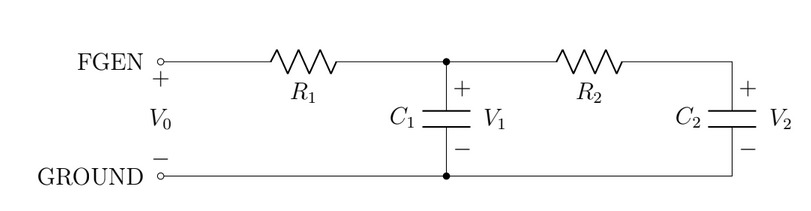
\includegraphics[scale=0.7]{figuras/figura1}
\end{table}

\begin{center}
Figura 1: Circuito em regime AC
\end{center}

\vspace{5pt}
\begin{table}[h]
\centering
\begin{tabular}{|c|c|c|c|}
\hline
\textbf{Grandeza} & \textbf{Valor calculado} & \textbf{Valor medido} & \textbf{Erro (\%) }\\\hline
Amplitude de $V_1$ (frequência $0,25kHz$) & 0,975V & 1,02V & 4,62 \\\hline
Amplitude de $V_1$ (frequência $0,5kHz$) & 0,910V & 0,999V & 9,78 \\\hline
Amplitude de $V_1$ (frequência $1kHz$) & 0,755V & 0,893V & 18,28 \\\hline
Amplitude de $V_1$ (frequência $2kHz$) & 0,544V & 0,574V & 5,51 \\\hline
Fase de $V_1$ em relação a $V_0$ (frequência $0,25kHz$) & -10,34\textdegree & -12,26\textdegree & 18,57\\\hline
Fase de $V_1$ em relação a $V_0$ (frequência $0,5kHz$) & -19,25\textdegree & -14,38\textdegree & 25,30\\\hline
Fase de $V_1$ em relação a $V_0$ (frequência $1kHz$) & -32,24\textdegree & -17,30\textdegree & 46,34\\\hline
Fase de $V_1$ em relação a $V_0$ (frequência $2kHz$) & -42,47\textdegree & -46,07\textdegree & 8,48\\\hline
\end{tabular}
\caption*{Tabela 2: Tensões no capacitor $C_1$}
\end{table}
\vspace{5pt}
\begin{table}[h]
\centering
\begin{tabular}{|c|c|c|c|}
\hline
\textbf{Grandeza} & \textbf{Valor nominal} & \textbf{Valor medido} & \textbf{Erro (\%) }\\\hline
Amplitude de $V_2$ (frequência $0,25kHz$) & 0,972V & 1,02V & 4,94 \\\hline
Amplitude de $V_2$ (frequência $0,5kHz$) & 0,897V & 0,935V & 4,24 \\\hline
Amplitude de $V_2$ (frequência $1kHz$) & 0,711V & 0,744V & 4,64 \\\hline
Amplitude de $V_2$ (frequência $2kHz$) & 0,441V & 0,489V & 10,88 \\\hline
Fase de $V_2$ em relação a $V_0$ (frequência $0,25kHz$) & -15,45\textdegree & -18,74\textdegree & 21,29\\\hline
Fase de $V_2$ em relação a $V_0$ (frequência $0,5kHz$) & -29,88\textdegree & -38,90\textdegree & 30,19\\\hline
Fase de $V_2$ em relação a $V_0$ (frequência $1kHz$) & -52,08\textdegree & -57,58\textdegree & 10,56\\\hline
Fase de $V_2$ em relação a $V_0$ (frequência $2kHz$) & -78,36\textdegree & -80,62\textdegree & 2,88\\\hline
\end{tabular}
\caption*{Tabela 3: Tensão no capacitor $C_2$}
\end{table}

\section{Conclusão}

\section{Bibliografia}

\end{document}